\documentclass[areasetadvanced]{scrartcl}

\usepackage[utf8]{inputenc}
\usepackage[T2A]{fontenc}
\usepackage[english,russian]{babel}

\usepackage[footskip=1cm,left=25mm, right=15mm, top=20mm, bottom=20mm]{geometry}
\usepackage{setspace}
\usepackage{amsmath, amssymb}  % Объединено в одну строку
\usepackage{graphicx}
\usepackage{tikz}
\usetikzlibrary{arrows.meta}
\usepackage{float}
\usepackage{dashrule}
\usepackage{fancyhdr} % оформление отчёта
\usepackage{hyperref} % оформление отчёта
\usepackage{parskip}
\usepackage{textcomp, enumitem}
\usepackage{indentfirst}
\usepackage{graphicx}
\usepackage{algorithm}
\usepackage{algpseudocode}
\usepackage{array}  % Для использования команды m{}
\usepackage{geometry}
\usepackage{afterpage}
\usepackage{minted}
\setcounter{secnumdepth}{3}  % Включает нумерацию для subsubsection
\setcounter{tocdepth}{3}     % Включает subsubsection в содержание
\usepackage{listings} % Если используете listings
\setlength{\parindent}{1.25cm} % ГОСТовский отступ
\tikzstyle{block} = [rectangle, rounded corners, minimum width=3cm, minimum height=1cm, text centered, draw=black, fill=lightgray]

\setkomafont{sectioning}{\normalfont\bfseries} % для заголовков разделов и подразделов
\setkomafont{section}{\normalfont\Large\bfseries}
\setkomafont{subsection}{\normalfont\large\bfseries}
\setkomafont{subsubsection}{\normalfont\large\bfseries}
\setkomafont{paragraph}{\normalfont\large\bfseries} % для заголовков параграфов (если они есть)

\lstset{
  language=Haskell,
  basicstyle=\ttfamily\small,
  keywordstyle=\color{blue}\bfseries,
  stringstyle=\color{red},
  commentstyle=\color{green!70!black},
  numbers=left,
  numberstyle=\tiny,
  stepnumber=1,
  numbersep=10pt,
  showstringspaces=false,
  breaklines=true,
  frame=single
}

\setcounter{tocdepth}{2}
\begin{document}
\sloppy
	\thispagestyle{empty}
	\begin{center}
		\large{МИНОБРНАУКИ РОССИИ} \par
		\vspace{0.3cm}
		\normalsize
		{ФЕДЕРАЛЬНОЕ ГОСУДАРСТВЕННОЕ АВТОНОМНОЕ ОБРАЗОВАТЕЛЬНОЕ УЧРЕЖДЕНИЕ ВЫСШЕГО ОБРАЗОВАНИЯ} \par
		\vspace{0.3cm}
		\textbf{\guillemotleft САНКТ-ПЕТЕРБУРГСКИЙ ПОЛИТЕХНИЧЕСКИЙ}
		\textbf{УНИВЕРСИТЕТ ПЕТРА ВЕЛИКОГО\guillemotright} \par
		\vspace{0.3cm}
		{Институт компьютерных наук и кибербезопасности}\par
		{Высшая школа технологий искусственного интеллекта}\par
	\end{center}
	\vfill
	\begin{center}
		{\large Отчёт по дисциплине \guillemotleft Алгоритмические основы компьютерной графики\guillemotright}\par
		{\huge   Лабораторная работа №1 
		
		\guillemotleft Технологии построения реалистических моделей в Blender\guillemotright}\par
        
	\end{center}
	\vfill
	\begin{flushleft}
		Студент: \hspace{1.8cm} \rule[0pt]{2.5cm}{0.5pt}\hfill Салимли Айзек Мухтар Оглы\par
		\vspace{1.5cm}
		Преподаватель: \hspace{0.55cm} \rule[0pt]{2.5cm}{0.5pt}\hfill  Курочкин Михаил Александрович
	\end{flushleft}
	\vspace{0.5cm}
	\begin{flushright}
		\guillemotleft \rule[0pt]{0.8cm}{0.5pt}\guillemotright \rule[0pt]{2cm}{0.5pt} 20\rule[0pt]{0.5cm}{0.5pt} г.
	\end{flushright}
	\vfill
	\begin{center}
		Санкт-Петербург, 2025
	\end{center}
	\newpage
	\tableofcontents
	\newpage
\section*{Введение}
	\addcontentsline{toc}{section}{Введение}
    Компьютерная графика позволяет создавать максимально реалистичные модели
    объекта. Сегодня 3D-моделирование используется в проектировании зданий, в ландшафтном
    дизайне, дизайне интерьеров, а также в компьютерных играх и программах, в
    промышленности и медицине, а также во многих других сферах. Важную роль 3D-
    моделирование играет при проведении презентации и демонстрации какого-либо продукта
    или услуги. Также 3D моделирование, анимация и визуализация объектов играет важную
    роль в современном мире при реализации различных бизнес-процессов и успешном
    взаимодействии с заказчиком. Требования к созданию 3D модели, на данный момент, очень
    высоки. Трехмерное моделирование дает очень точную модель, максимально приближенную
    к реальности. 

    Современные программы помогают достичь высокой детализации. При этом
    значительно увеличивается наглядность проекта. Выразить трехмерный объект в двухмерной
    плоскости не просто, тогда как 3D визуализации дает возможность тщательно проработать и
    что самое главное, просмотреть все детали. Это более естественный способ визуализации.
    Профессиональные программы дают множество преимуществ и изготовителю. 

    Из трехмерной модели легко можно выделить чертеж каких-либо компонентов или конструкции
    целиком. Несмотря на то, что создание трехмерной модели довольно трудозатратный
    процесс, работать с ним в дальнейшем гораздо проще и удобнее чем с традиционными
    чертежами. В результате значительно сокращаются временные затраты на проектирование,
    снижаются издержки.

        Проблемой является алгоритмическая сложность при учёте всех физических законов,
    которые влияют на внешнее восприятие действительности. Основные влияющие факторы:
    распределения световой энергии в пространстве, её диффузии и отражении от тел,
    проявление свойств интерференции, дифракции света, и прочее. В зависимости от
    требований к качеству изображения предъявляются и требования к качеству визуализации и
    могут учитываться различные физические законы. 
    
        Для создания 3D моделей была выбрана среда Blender. Blender — профессиональное
    cвободное и открытое программное обеспечение для создания трёхмерной компьютерной
    графики, включающее в себя средства моделирования, скульптинга и анимации.
\newpage
\section{Постановка задачи}
В лабораторной работе №1 требуется:
\begin{enumerate}
    \item Ознакомится с возможностями пакета Blender, которые позволяют создавать реалистичные модели реальный объектов.
    \item Выбрать три объекта реального мира и построить их реалистичную модель в пакете Blender с учетом уникальных особенностей моделируемого объекта
    \item Отразить характерные особенности объекта, такие как:
    \subitem - Геометрическая форма
    \subitem - Материал
    \subitem - Текстура
    \subitem - Царапины и иные особенности объекта
    \item Предоставить пошаговое руководство пользователя по получению результата
\end{enumerate}
\newpage
\section{Описание функциональных возможностей пакета Blender}
\begin{center}
    \textbf{Функции пакета}
\end{center}
\begin{itemize}
\item Поддержка разнообразных геометрических примитивов, включая полигональные модели,
систему быстрого моделирования в режиме subdivision surface (SubSurf), кривые Безье,
поверхности NURBS, metaballs (метасферы), скульптурное моделирование и векторные
шрифты.
\item Универсальные встроенные механизмы рендеринга и интеграция с внешними рендерерами
YafRay, LuxRender и многими другими.
\item Инструменты анимации, среди которых инверсная кинематика, скелетная анимация и
сеточная деформация, анимация по ключевым кадрам, нелинейная анимация,
редактирование весовых коэффициентов вершин, ограничители.
\item Динамика мягких тел (включая определение коллизий объектов при взаимодействии),
динамика твёрдых тел на основе физического движка Bullet.
\item Система частиц включающая в себя систему волос на основе частиц.
\item Модификаторы для применения неразрушающих эффектов.
\item Язык программирования Python используется как средство определения интерфейса,
создания инструментов и прототипов, системы логики в играх, как средство импорта/
экспорта файлов (например, COLLADA), автоматизации задач.
\item Базовые функции нелинейного видео и аудио монтажа.
\item Композитинг видео, работа с хромакеем.
\item Трекинг камеры и объектов.
\item Real-time контроль во время физической симуляции и рендеринга.
\item Процедурное и node-based текстурирование, а также возможность рисовать текстуру прямо
на модели.
\end{itemize}
\begin{center}
    \textbf{Отличительные особенности интерфейса пользователя}
\end{center}
\begin{itemize}
    \item Режимы редактирования. Два основных режима Объектный режим (Object mode) и Режим
редактирования (Edit mode), которые переключаются клавишей Tab. Объектный режим в
основном используется для манипуляций с индивидуальными объектами, в то время как
режим редактирования — для манипуляций с фактическими данными объекта. К примеру,
для полигональной модели в объектном режиме мы можем перемещать, изменять размер и
вращать модель целиком, а режим редактирования используется для манипуляции
отдельных вершин конкретной модели. Также имеются несколько других режимов, таких
как Sculpting, Texture Paint, Vertex Paint и UV Face select.
\item Широкое использование горячих клавиш. Большинство команд выполняется с клавиатуры.
До появления 2.x и особенно 2.3x-версии, это был единственный путь выполнять команды,
и это было самой большой причиной создания репутации Blender’y как сложной для
изучения программы. Новая версия имеет более полное графическое меню.
\item Управление рабочим пространством. Графический интерфейс Blender-а состоит из одного
или нескольких экранов, каждый из которых может быть разделён на секции и подсекции,
которые могут быть любой частью интерфейса Blender’a. Графические элементы каждой
секции могут контролироваться теми же инструментами, что и для манипуляции в 3D-
пространстве, для примера можно уменьшать и увеличивать кнопки инструментов тем же
путём, что и в 3D-просмотре.
\end{itemize}
\newpage 
\section{Описание объектов моделирования}
\subsection{Первый моделируемый объект}
\begin{itemize}
    \item Наименование объекта: Карандаш.
	\item Особенности: \begin{enumerate}
        \item Материал: ДСП
        \item Цвета: кончик - черный, кантовка - белый, корпус - белый, головка - древесный, стержень - графитовый
        \item Заточка
        \item Потертая надпись
        \item Вмятина на конце корпуса
    \end{enumerate}
\end{itemize}
Фото моделируемого объекта: %%%%%%%%%%%%%%%%%%%%%%%%%%%% ФОТО
\begin{figure}[H]
    \centering
    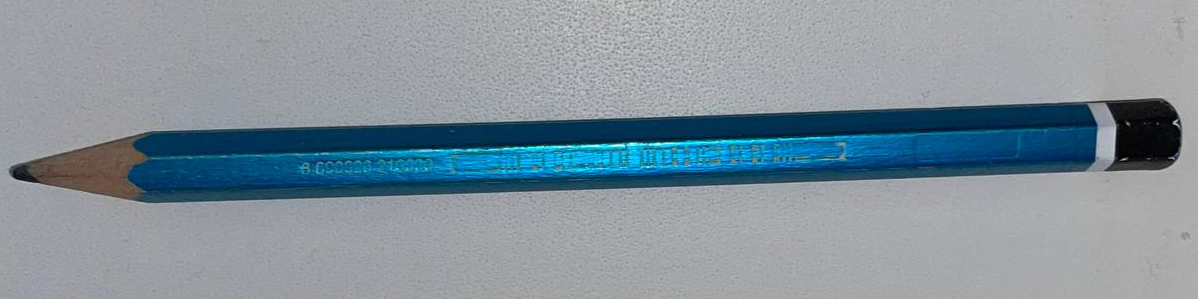
\includegraphics[width=0.5\textwidth]{PencilName.png}
    \caption{Фронтальная часть карандаша (потертая запись)}
    \label{fig:syntdiag}
\end{figure}

\subsection{Второй моделируемый объект}
\begin{itemize}
    \item Наименование объекта: Колпак от авторучки.
	\item Особенности: \begin{enumerate}
        \item Материал: Пластик
        \item Цвета: Синий
        \item Согнутый держатель 
        \item Надпись
        \item Усеченный кончик держателя
    \end{enumerate}
\end{itemize}
Фото моделируемого объекта:
\begin{figure}[H]
    \centering
    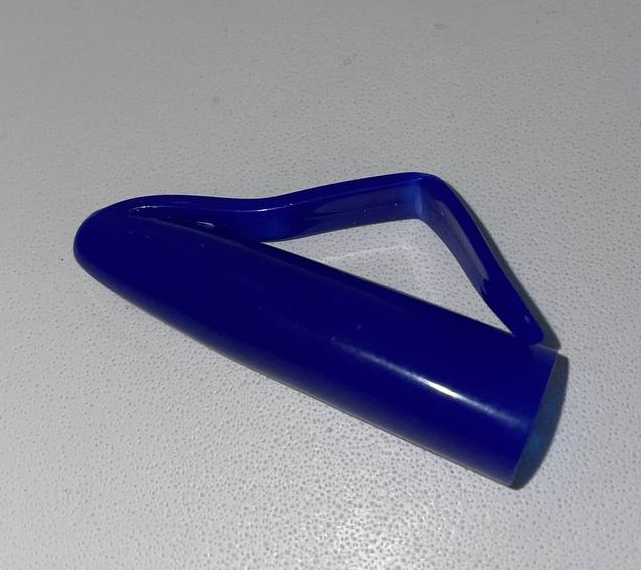
\includegraphics[width=0.5\textwidth]{Kolpak_org.png}
    \caption{Колпак от авторучки с согнутым держателем.}
    \label{fig:syntdiag}
\end{figure}
\begin{figure}[H]
    \centering
    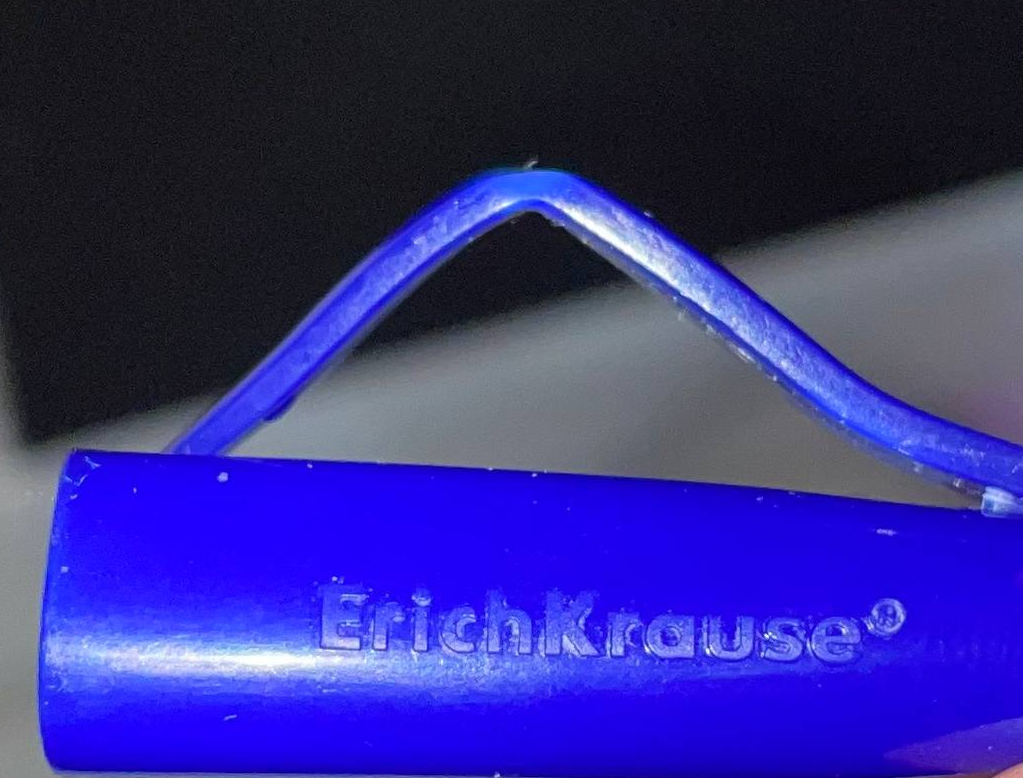
\includegraphics[width=0.5\textwidth]{KolpakName.png}
    \caption{Надпись на колпаке от авторучки.}
    \label{fig:syntdiag}
\end{figure}
\begin{figure}[H]
    \centering
    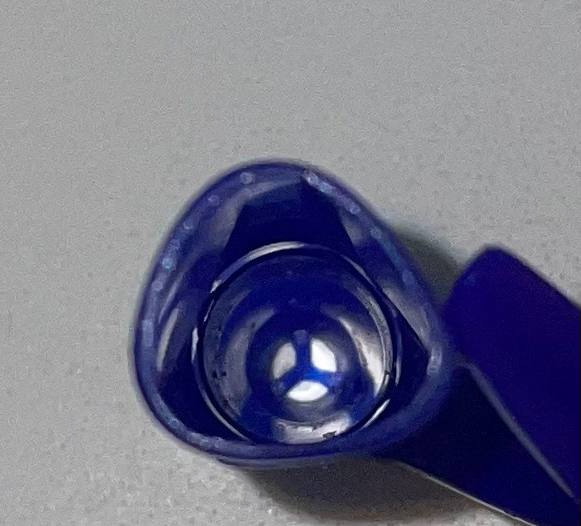
\includegraphics[width=0.5\textwidth]{KolpakBottom.png}
    \caption{Задняя часть колпака от авторучки.}
    \label{fig:syntdiag}
\end{figure}
\subsection{Третий моделируемый объект}
\begin{itemize}
    \item Наименование объекта: Игрушечный динозавр.
	\item Особенности: \begin{enumerate}
        \item Материал: Пластик
        \item Цвета: Фронтальный вид: Черный + белые кости, Задний вид: светло-зеленный
        \item Поттертости сзади
        \item Поттертость на голове динозавра
        \item Объект находится в единственном экземпляре и сделан собственноручно
    \end{enumerate}
\end{itemize}
Фото моделируемого объекта:
\begin{figure}[H]
    \centering
    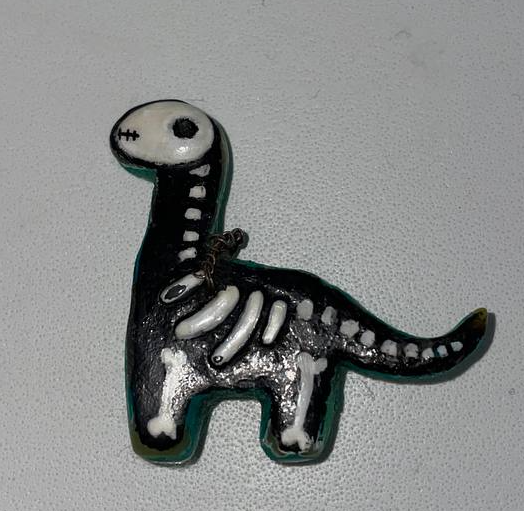
\includegraphics[width=0.5\textwidth]{DinoFront.png}
    \caption{Передняя часть динозавра.}
    \label{fig:syntdiag}
\end{figure}
\begin{figure}[H]
    \centering
    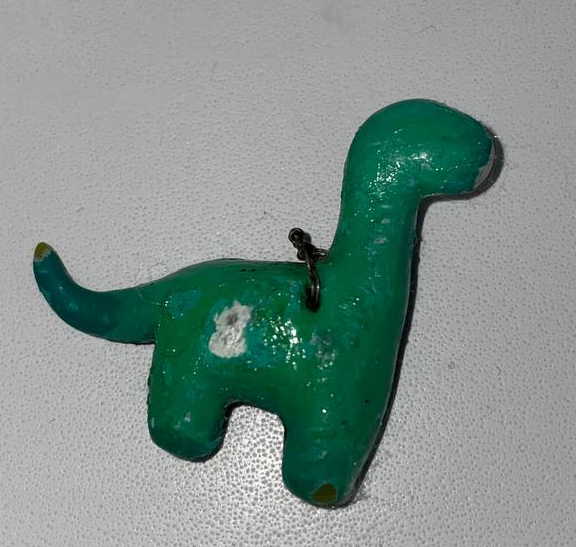
\includegraphics[width=0.5\textwidth]{DinoBack.png}
    \caption{Задняя часть динозавра.}
    \label{fig:syntdiag}
\end{figure}

\newpage
\section{Процесс моделирования}

\subsection{Процесс моделирования 1-го объекта}
\subsubsection{Построение геомтерической модели}
\par \textbf{Шаг 1:} Открываем меню Добавить объект \textit{Shift + A -> Mesh ->  Cylinder}.
\begin{figure}[H]
    \label{4} 
    \centering
    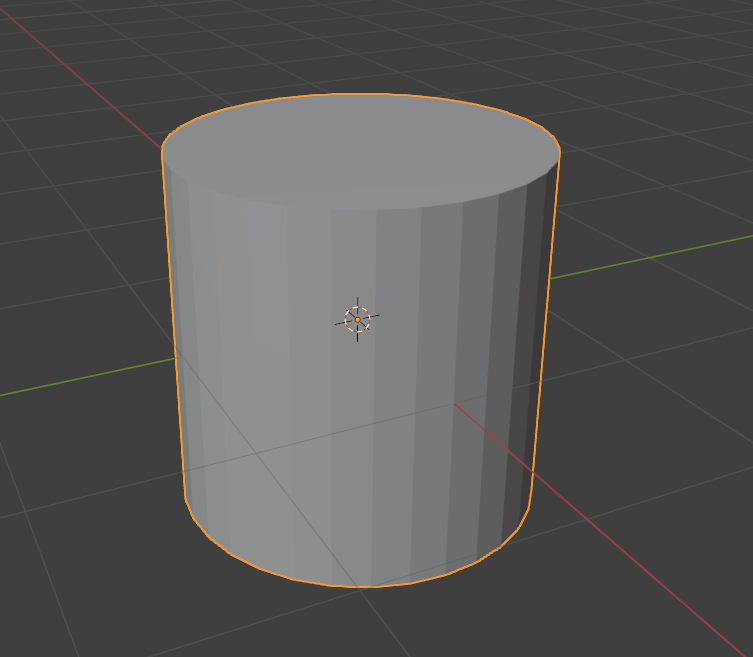
\includegraphics[width=0.6\linewidth]{pen/1.png}
    \caption{Шаг 1}
\end{figure}

\par \textbf{Шаг 2:} Задаём ему следующие параметры, чтобы придать форму карандаша.
\begin{figure}[H]
    \label{4} 
    \centering
    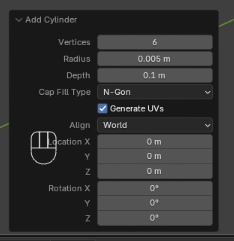
\includegraphics[width=0.5\linewidth]{pen/2.png}
    \caption{Шаг 2}
\end{figure}


\par \textbf{Шаг 3:} Выбираем грани фигуры и с помощью инструмента Subdivide (\textit{ПКМ -> Subdivide}) добавляем рёбро для ограничения деревянной части карндаша.
\par Параметры Subdivide:
\begin{itemize}
    \item Number of Cuts: 1
    \item Smoothness: 0
\end{itemize}

\begin{figure}[H]
    \label{4} 
    \centering
    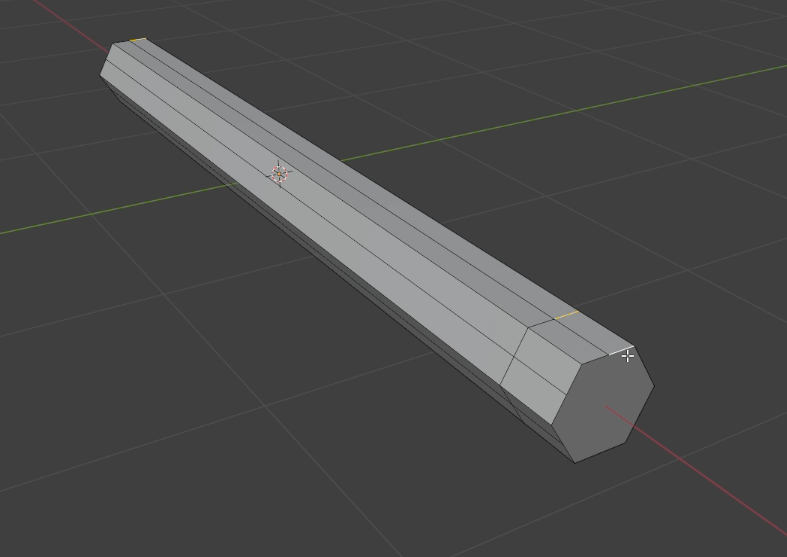
\includegraphics[width=0.6\linewidth]{pen/3.png}
    \caption{Шаг 3}
\end{figure}


\par \textbf{Шаг 4:} Выделяем все крайние вершины у деревянной части и с помощью инструмента Merge (\textit{клавиша M}) соединяем их.
\begin{figure}[H]
    \label{4} 
    \centering
    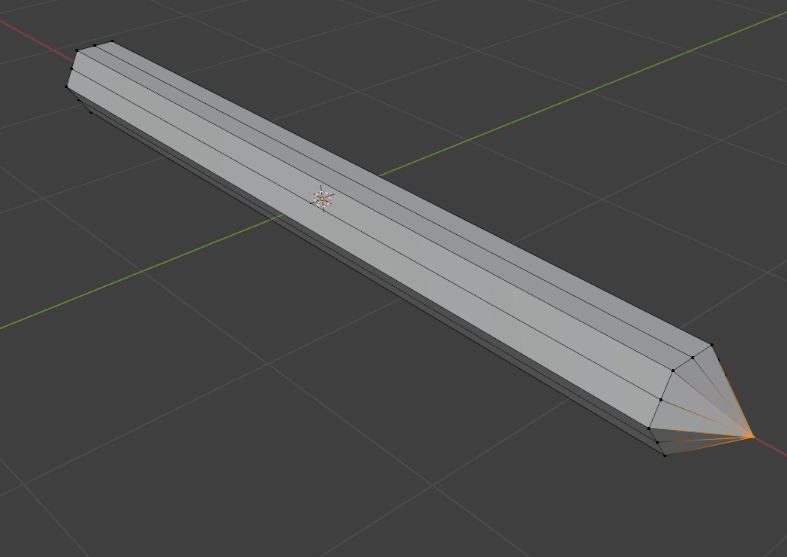
\includegraphics[width=0.6\linewidth]{pen/4.png}
    \caption{Шаг 4}
\end{figure}


\par \textbf{Шаг 5:} Выделяем вершины на деревянной части карандаша. Для снятия фаски с этих вершин необходимо нажать комбинацию клавиш \textit{Ctrl+B} и задать следующие параметры:
\begin{itemize}
    \item Width: 2m
    \item Segments: 20
    \item Shape: 0.5
\end{itemize}

\begin{figure}[H]
    \label{4} 
    \centering
    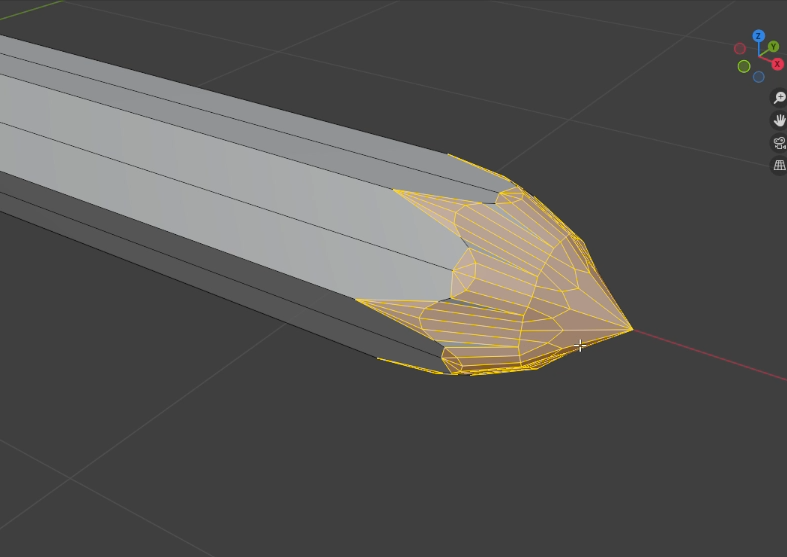
\includegraphics[width=0.6\linewidth]{pen/5.png}
    \caption{Шаг 5}
\end{figure} 


\par \textbf{Шаг 6:} Выбираем грани фигуры и с помощью инструмента Subdivide (\textit{ПКМ -> Subdivide}) добавляем 2 рёбра для ограничения части карндаша чёрного цвета.
\par Параметры Subdivide:
\begin{itemize}
    \item Number of Cuts: 2
    \item Smoothness: 0
\end{itemize}

\begin{figure}[H]
    \label{4} 
    \centering
    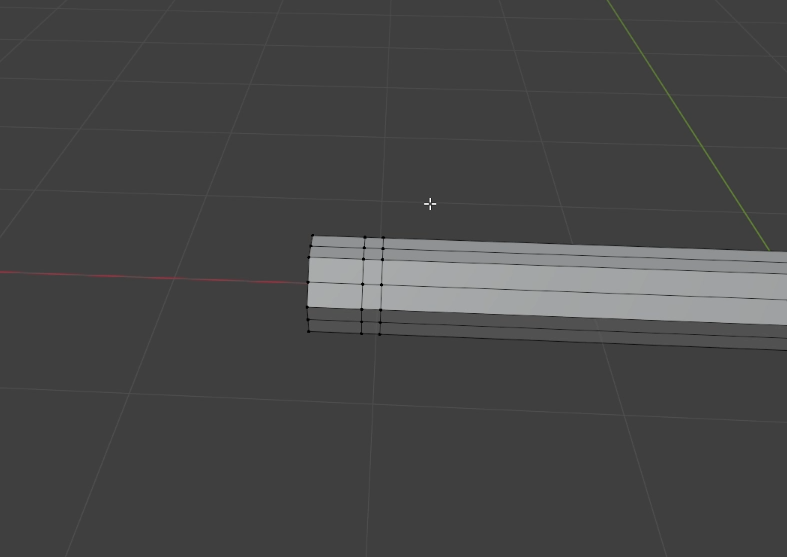
\includegraphics[width=0.6\linewidth]{pen/6.png}
    \caption{Шаг 6}
\end{figure}


\par \textbf{Шаг 7:} Выделяем вершины на крайней части карандаша. Для придания более плавных форм и снятия фаски с этих вершин необходимо нажать комбинацию клавиш \textit{Ctrl+B} и задать следующие параметры:
\begin{itemize}
    \item Width: 1m
    \item Segments: 10
    \item Shape: 0.5
\end{itemize}

\begin{figure}[H]
    \label{4} 
    \centering
    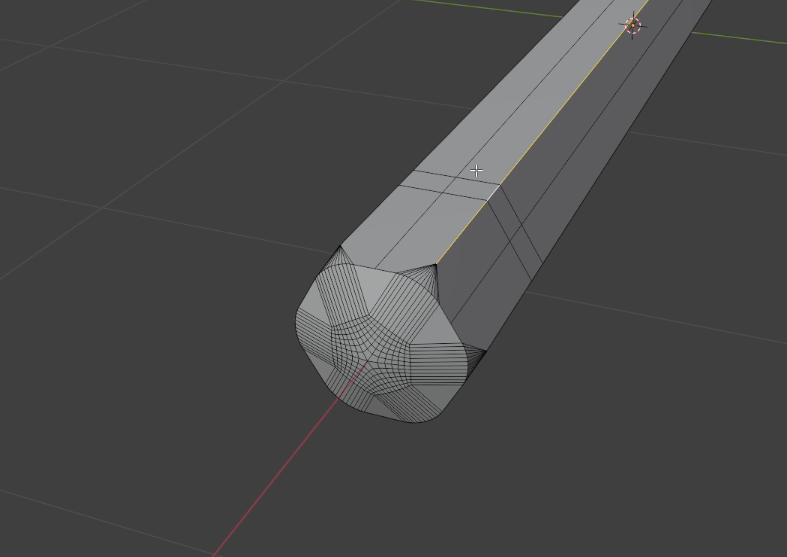
\includegraphics[width=0.6\linewidth]{pen/7.png}
    \caption{Шаг 7}
\end{figure} 


\par \textbf{Шаг 8:} Выделяем боковые грани карандаша. Для и снятия фаски с этих ребёр необходимо нажать комбинацию клавиш \textit{Ctrl+B} и задать следующие параметры:
\begin{itemize}
    \item Width: 0.5m
    \item Segments: 5
    \item Shape: 0.5
\end{itemize}

\begin{figure}[H]
    \label{4} 
    \centering
    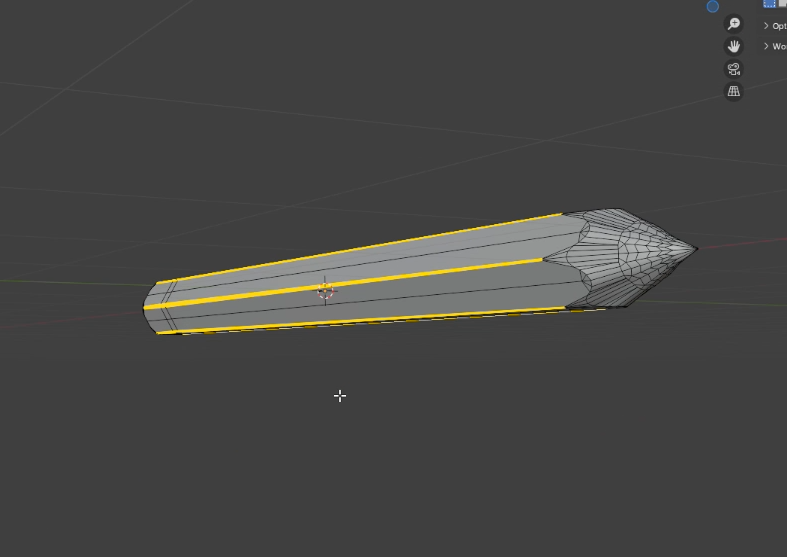
\includegraphics[width=0.6\linewidth]{pen/8.png}
    \caption{Шаг 8}
\end{figure} 



\par \textbf{Шаг 9:} Для добавления надписи на карандаш необходимо открыть меню Добавить объект \textit{Shift + A -> Text}. Задаём текст \guillemotleft 8 690823 210000\guillemotright. Перемещаем надпись к верхней грани карандаша с помощью комбинации клавиш \textit{G+Z}.
\begin{figure}[H]
    \label{4} 
    \centering
    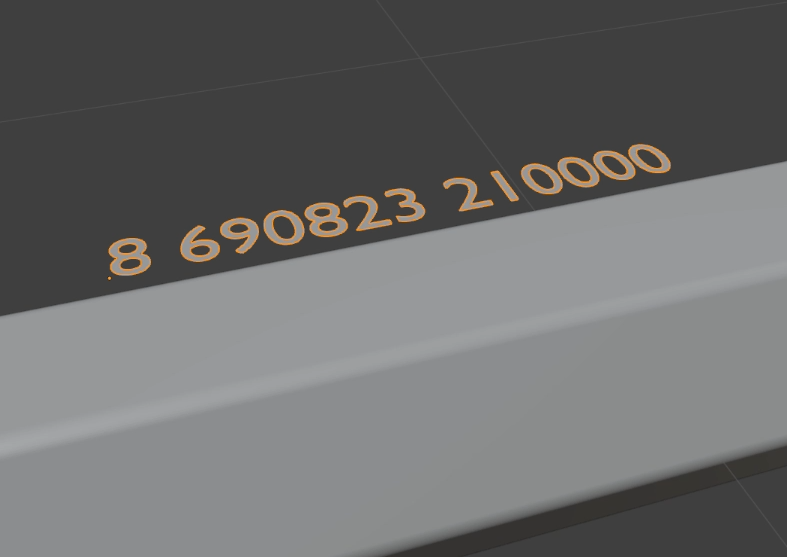
\includegraphics[width=0.6\linewidth]{pen/9.png}
    \caption{Шаг 9}
\end{figure}


\par \textbf{Шаг 10:} Для придания тексту объёма применяем на него модификатор Extrude (клавиша \textit{E}).
\par Параметры модификатора:
\begin{itemize}
    \item Move X: 0
    \item Move Y: 0
    \item Move Z: 0.1m
\end{itemize}

\begin{figure}[H]
    \label{4} 
    \centering
    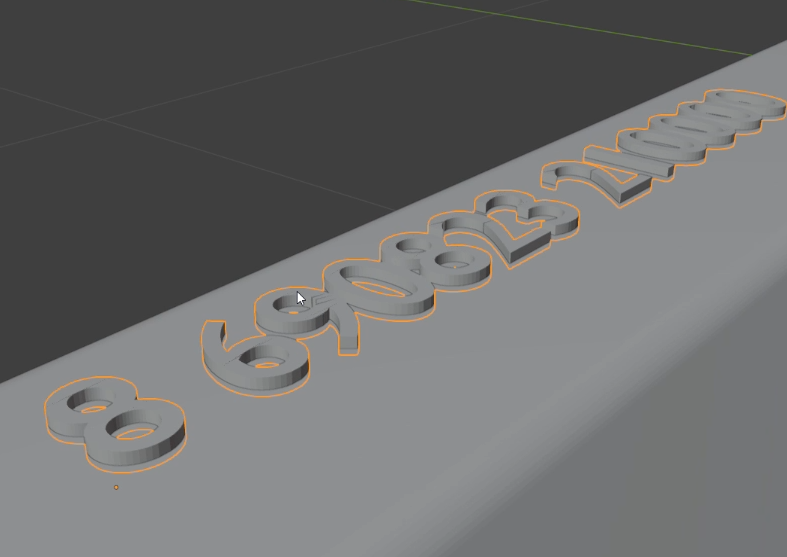
\includegraphics[width=0.6\linewidth]{pen/10.png}
    \caption{Шаг 10}
\end{figure}


\par \textbf{Шаг 11:} Для создания объёмной надписи на карандаше необходимо применить к тексту и карандашу модификатор Boolean (Difference).
\begin{figure}[H]
    \label{4} 
    \centering
    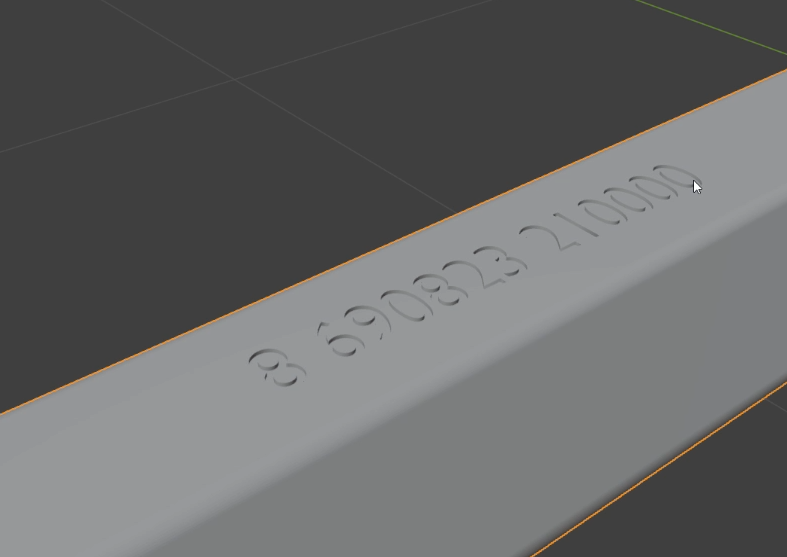
\includegraphics[width=0.6\linewidth]{pen/11.png}
    \caption{Шаг 11}
\end{figure}


\par \textbf{Шаг 12:} Для работы со скульптингом данной модели необходимо перейти в режим отображения \textit{Sculpting} и применить инструмент \textit{Remesh} с целью уплотнения сетки со следующим параметром:
\begin{itemize}
    \item Voxel Size: 0.003m
\end{itemize}
\begin{figure}[H]
    \label{4}  
    \centering
    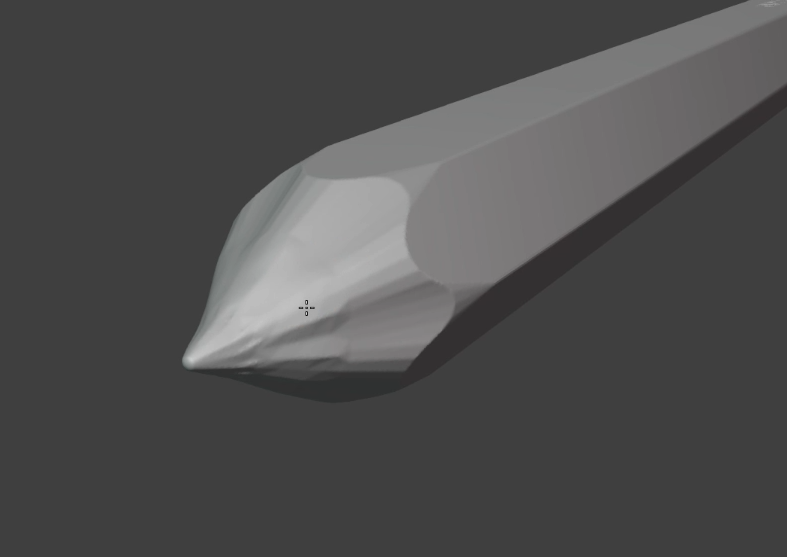
\includegraphics[width=0.6\linewidth]{pen/12.png}
    \caption{Шаг 12}
\end{figure}


\par \textbf{Шаг 13:} Затем, для создания царапин на модели необходимо выбрать инструмент \textit{Draw} с параметрами:
\begin{itemize}
    \item Radius: 42px
    \item Strength: 0.257
    \item Direction: Add
\end{itemize}
\par и с помощью нажатий \textit{ЛКМ} добавляем царапины на модель
\begin{figure}[H]
    \label{4}  
    \centering
    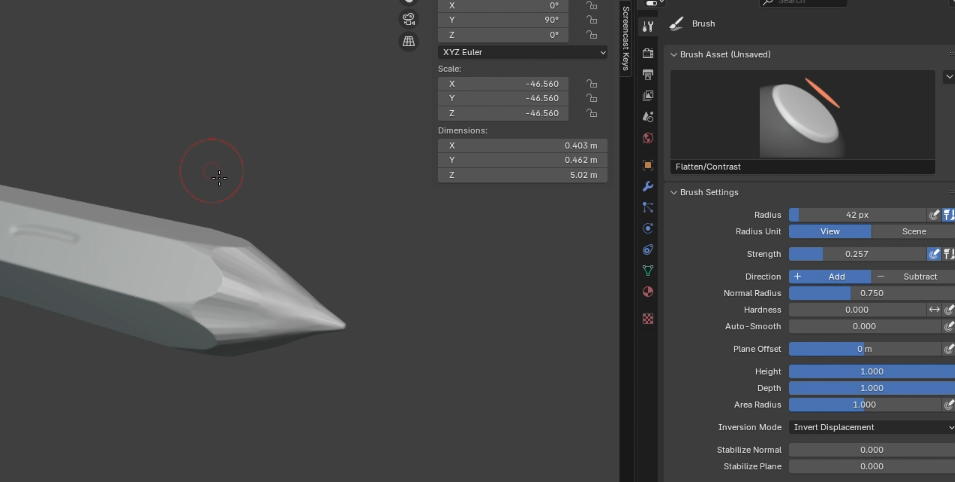
\includegraphics[width=0.8\linewidth]{pen/13.png}
    \caption{Шаг 13}
\end{figure}


\subsubsection{Добавление материала}
\par \textbf{Шаг 1:} Выбираем режим отображения Shading для Blender, чтобы перейти в режим редактирования материалов. Для каждого отдельного материала необходимо задать цвет максимально приближенный к исходному и следующие параметры:

\par \textbf{Тело карандаша}
\begin{enumerate}
    \item Metallic: 0.0
    \item Roughness: 0.582
    \item IOR: 1.5
\end{enumerate}

\begin{figure}[H]
    \label{4} 
    \centering
    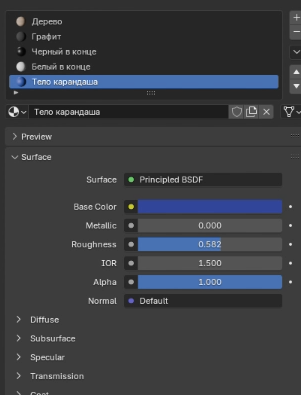
\includegraphics[width=0.4\linewidth]{pen/14.png}
\end{figure}

\par \textbf{Дерево}
\begin{enumerate}
    \item Metallic: 0
    \item Roughness: 1
    \item IOR: 1.5
\end{enumerate}

\begin{figure}[H]
    \label{4} 
    \centering
    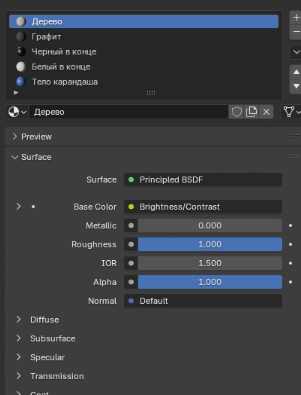
\includegraphics[width=0.4\linewidth]{pen/15.png}
\end{figure}

\par \textbf{Графит}
\begin{enumerate}
    \item Metallic: 0
    \item Roughness: 1
    \item IOR: 1.5
\end{enumerate}

\begin{figure}[H]
    \label{4} 
    \centering
    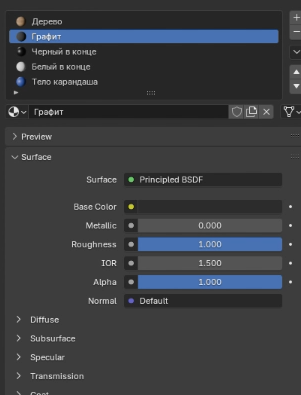
\includegraphics[width=0.4\linewidth]{pen/16.png}
\end{figure}

\par \textbf{Черный в конце}
\begin{enumerate}
    \item Metallic: 0
    \item Roughness: 0.418
    \item IOR: 1.5
\end{enumerate}

\begin{figure}[H]
    \label{4} 
    \centering
    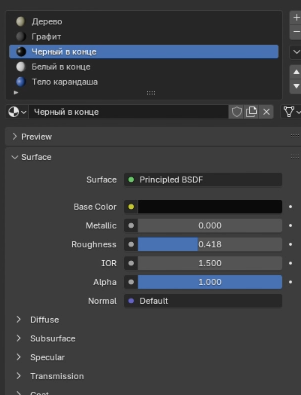
\includegraphics[width=0.4\linewidth]{pen/17.png}
\end{figure}

\par \textbf{Белый в конце}
\begin{enumerate}
    \item Metallic: 0
    \item Roughness: 0.514
    \item IOR: 1.5
\end{enumerate}

\begin{figure}[H]
    \label{4} 
    \centering
    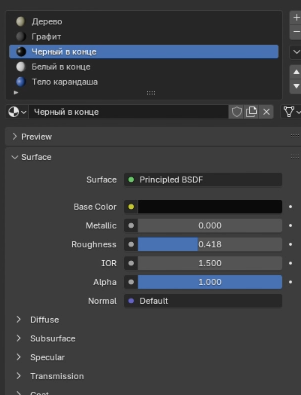
\includegraphics[width=0.4\linewidth]{pen/17.png}
\end{figure}






\newpage
\subsection{Процесс моделирования 2-го объекта}

\subsubsection{Построение геомтерической модели}
\par \textbf{Шаг 1:} Открываем меню Добавить объект \textit{Shift + A -> Mesh ->  Triangle}.
\begin{figure}[H]
    \label{4} 
    \centering
    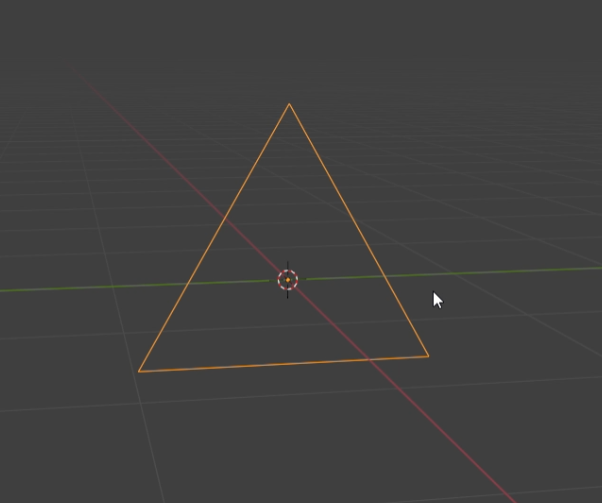
\includegraphics[width=0.6\linewidth]{col/1.png}
    \caption{Шаг 1}
\end{figure}


\par \textbf{Шаг 2:} Выделяем вершины треугольника. Для придания форму отверстия колпачка и снятия фаски с этих вершин необходимо нажать комбинацию клавиш \textit{Ctrl+B} и задать следующие параметры:
\begin{itemize}
    \item Width: 0.769m
    \item Segments: 16
    \item Shape: 0.5
\end{itemize}

\begin{figure}[H]
    \label{4} 
    \centering
    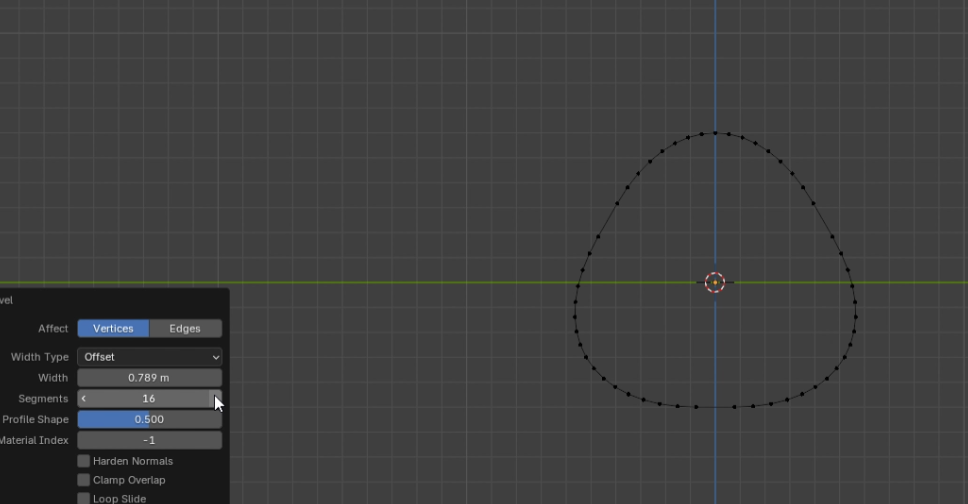
\includegraphics[width=0.6\linewidth]{col/2.png}
    \caption{Шаг 2}
\end{figure} 

\par \textbf{Шаг 3:} Дважды применяем модификатор Extrude (клавиша \textit{E}) для создания тела колпачка.
\par Параметры 1-го модификатора:
\begin{itemize}
    \item Move X: 2m
    \item Move Y: 0
    \item Move Z: 0
\end{itemize}
\par Параметры 2-го модификатора:
\begin{itemize}
    \item Move X: 0.5m
    \item Move Y: 0
    \item Move Z: 0
\end{itemize}
\begin{figure}[H]
    \label{4} 
    \centering
    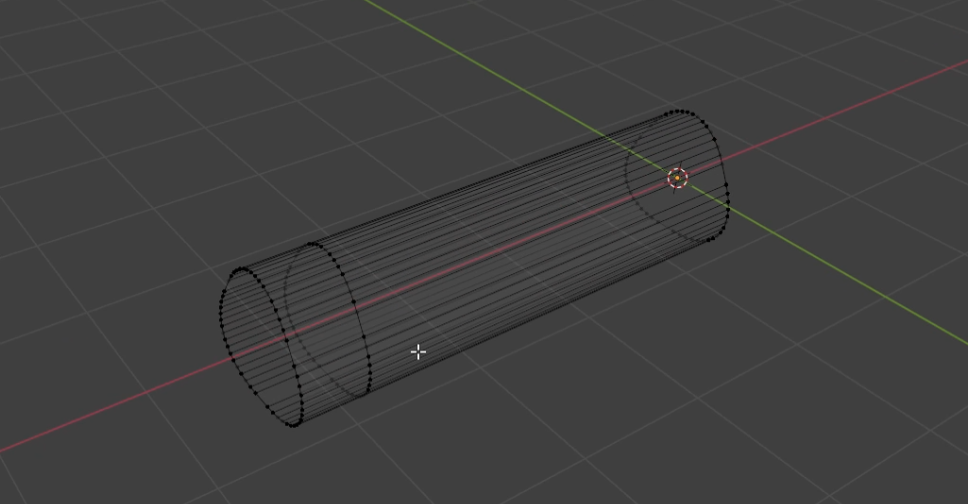
\includegraphics[width=0.6\linewidth]{col/3.png}
    \caption{Шаг 3}
\end{figure} 


\par \textbf{Шаг 4:} Выделяем вершины со стороны короткого отрезка колпачка. Для сужения этой части необходимо применить Scale (\textit{S}) и движением мыши уменьшить часть колпачка:

\begin{figure}[H]
    \label{4} 
    \centering
    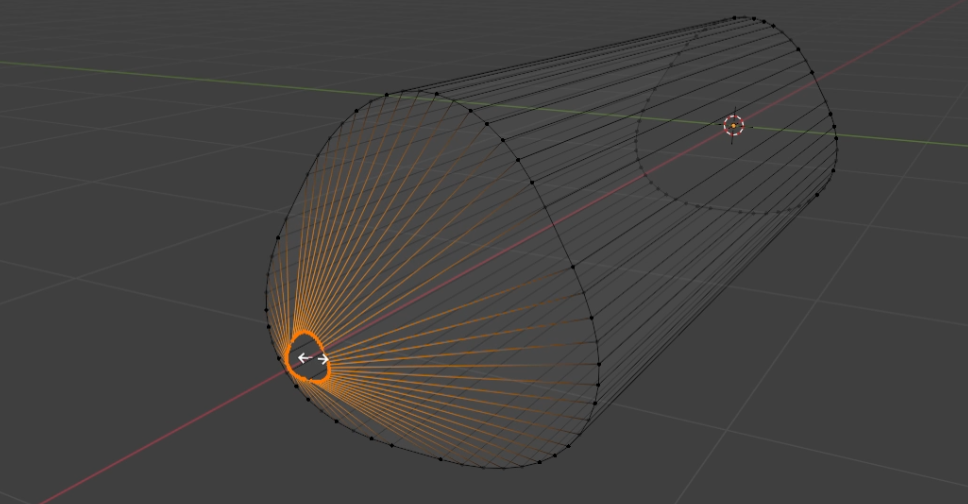
\includegraphics[width=0.6\linewidth]{col/4.png}
    \caption{Шаг 4}
\end{figure} 


\par \textbf{Шаг 5:} Выделяем вершины в середине колпачка. Для снятия фаски с этих ребёр необходимо нажать комбинацию клавиш \textit{Ctrl+B} и задать следующие параметры:
\begin{itemize}
    \item Width: 0.487m
    \item Segments: 21
    \item Shape: 0.5
\end{itemize}

\begin{figure}[H]
    \label{4} 
    \centering
    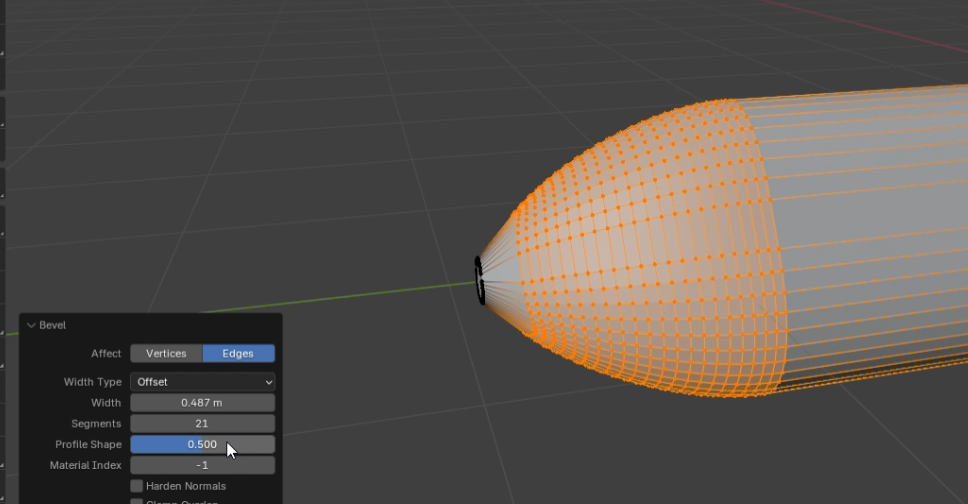
\includegraphics[width=0.6\linewidth]{col/5.png}
    \caption{Шаг 5}
\end{figure} 


\par \textbf{Шаг 6:} Выделяем открытую узкую часть колпачка. Для закрытия этого отвестия применяем инструмент Fill (\textit{Alt-F}):

\begin{figure}[H]
    \label{4} 
    \centering
    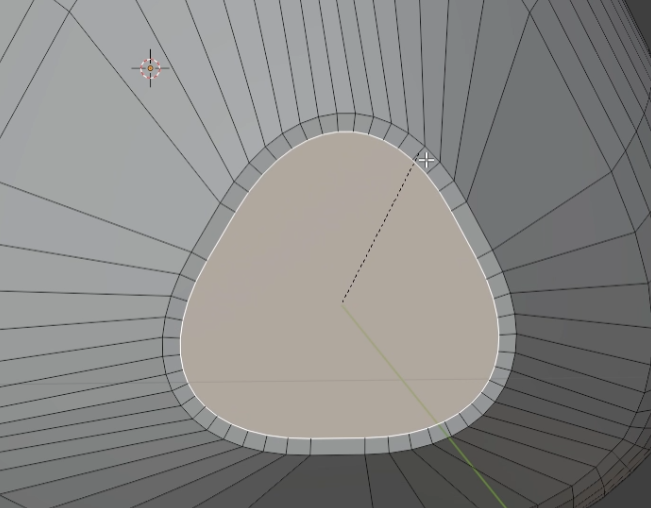
\includegraphics[width=0.6\linewidth]{col/6.png}
    \caption{Шаг 6}
\end{figure} 

\par \textbf{Шаг 7:} Для создания отвестий в этой части колпачка создаём треугольник \textit{Shift + A -> Mesh ->  Triangle}. С одной из вершин снимаем фаску \textit{Ctrl+B} и задать следующие параметры:
\begin{itemize}
    \item Width: 0.04m
    \item Segments: 5
    \item Shape: 0.5
\end{itemize}

Затем располагаем его у узкой части колпачка
\begin{figure}[H]
    \label{4} 
    \centering
    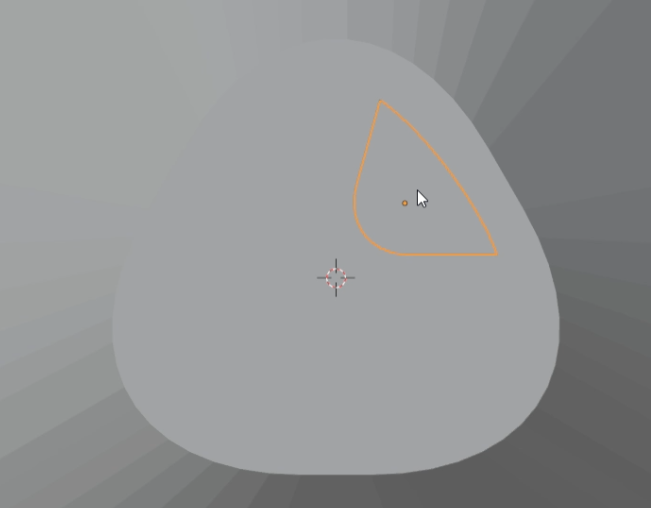
\includegraphics[width=0.6\linewidth]{col/7.png}
    \caption{Шаг 7}
\end{figure} 


\par \textbf{Шаг 8:} С помощью дублирования (\textit{Shift-D}) и вращения (\textit{R}) создаём ещё 2 копии этой фигуры:
\begin{figure}[H]
    \label{4} 
    \centering
    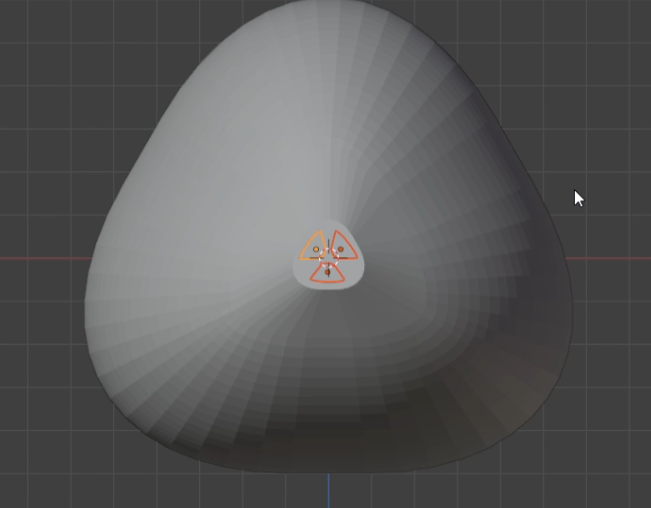
\includegraphics[width=0.6\linewidth]{col/8.png}
    \caption{Шаг 8}
\end{figure} 


\par \textbf{Шаг 9:} Для создания отверстий в колпачке необходимо применить к треугольникам и колпачку модификатор Boolean (Difference).
\begin{figure}[H]
    \label{4} 
    \centering
    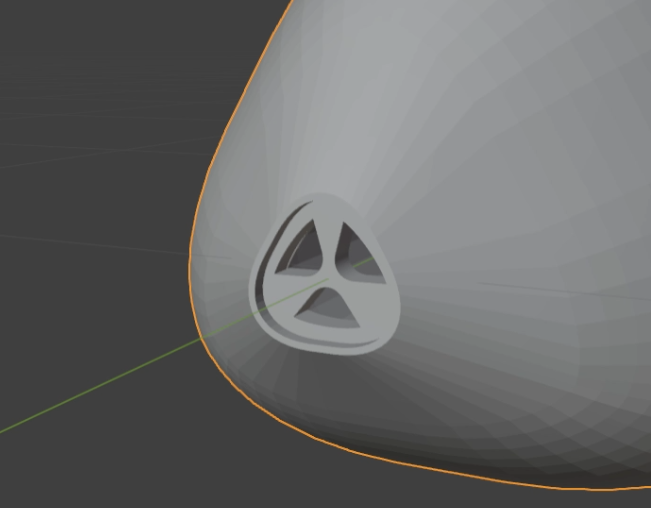
\includegraphics[width=0.6\linewidth]{col/9.png}
    \caption{Шаг 9}
\end{figure}


\par \textbf{Шаг 10:} Для создания изогнутого держателя колпачка создаём 2 кривые линии (\textit{Shift + A -> Mesh ->  Spline}).
\begin{figure}[H]
    \label{4} 
    \centering
    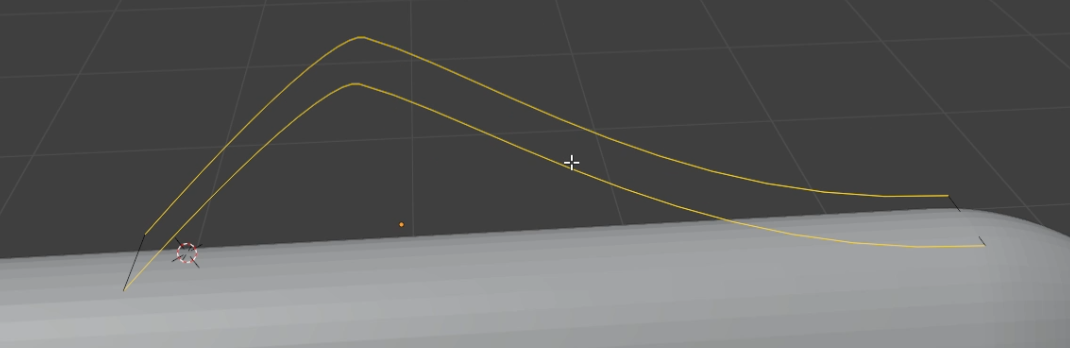
\includegraphics[width=0.6\linewidth]{col/10.png}
    \caption{Шаг 10}
\end{figure}


\par \textbf{Шаг 11:} Выделяем их обе и соединяем их поверхностью (\textit{Menu -> Edge -> Bridge Edge Loops}).
\begin{figure}[H]
    \label{4} 
    \centering
    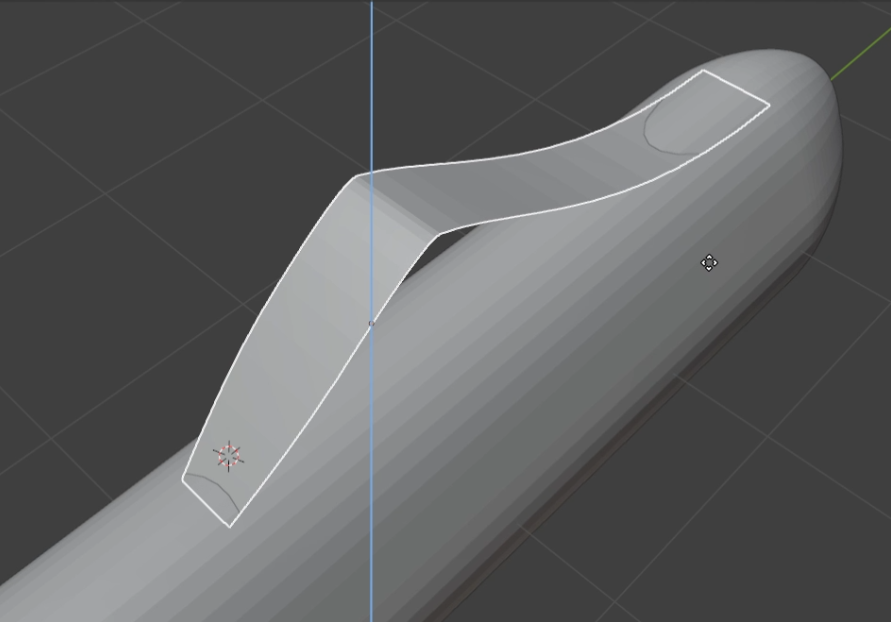
\includegraphics[width=0.6\linewidth]{col/11.png}
    \caption{Шаг 11}
\end{figure}


\par \textbf{Шаг 12:} Для создания искривления у держателя выделяем половину полигонов и поворачиваем их (\textit{R}).
\begin{figure}[H]
    \label{4} 
    \centering
    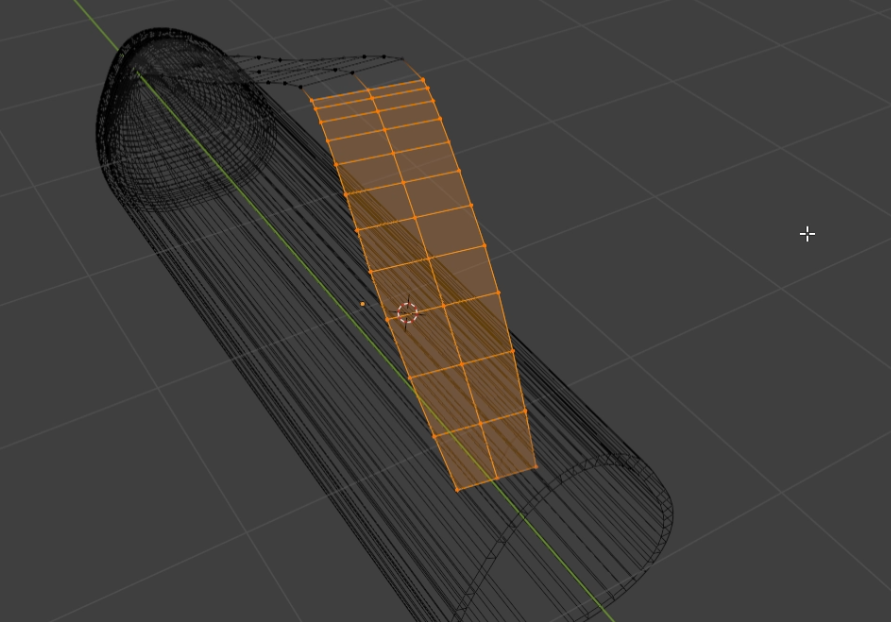
\includegraphics[width=0.6\linewidth]{col/12.png}
    \caption{Шаг 12}
\end{figure}


\par \textbf{Шаг 13:} Для добавления надписи на колпачок необходимо открыть меню Добавить объект \textit{Shift + A -> Text}. Задаём текст \guillemotleft ErichKrause®\guillemotright. Перемещаем надпись к боковой грани колпачка с помощью комбинации клавиш \textit{G+X}.
\begin{figure}[H]
    \label{4} 
    \centering
    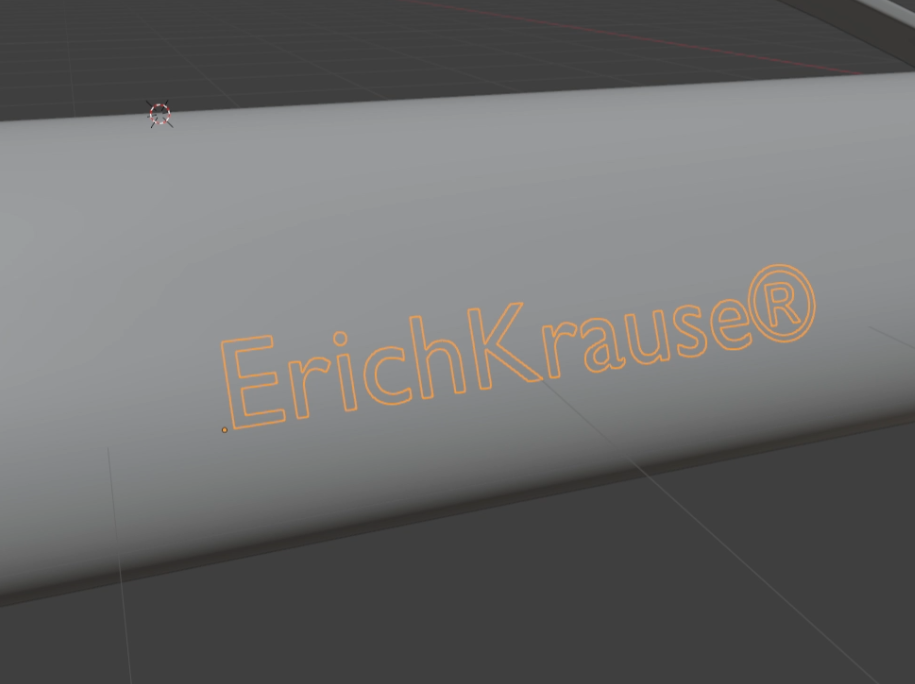
\includegraphics[width=0.6\linewidth]{col/13.png}
    \caption{Шаг 13}
\end{figure}


\par \textbf{Шаг 14:} Для придания тексту объёма применяем на него модификатор Extrude (\textit{E}).
\par Параметры модификатора:
\begin{itemize}
    \item Move X: 0
    \item Move Y: 0
    \item Move Z: 0.2m
\end{itemize}

\begin{figure}[H]
    \label{4} 
    \centering
    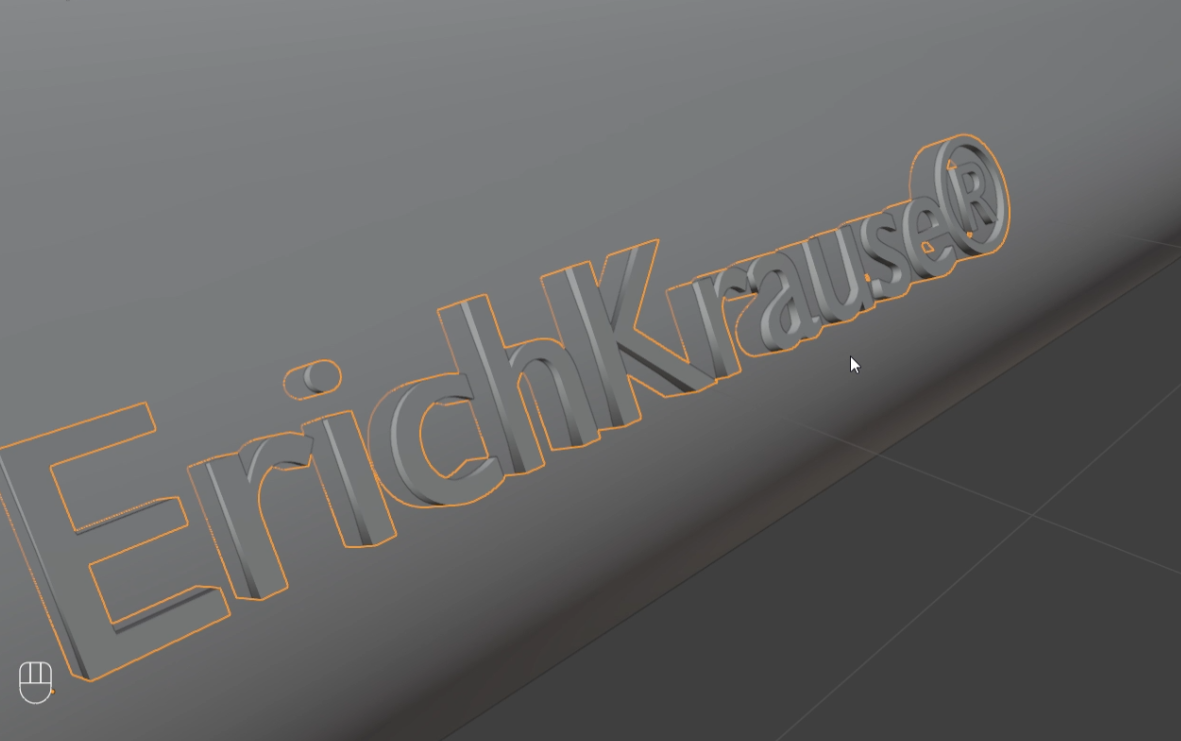
\includegraphics[width=0.6\linewidth]{col/14.png}
    \caption{Шаг 14}
\end{figure}

\subsubsection{Добавление материала}
\par \textbf{Шаг 1:} Переходим в «Material properties» на панели инструментов → во вкладку «surface» → «Base color» → в поле «Set color» выберем из представленных наиболее похожий цвет на оригинальный цвет объекта, и следующие параметры:
\begin{enumerate}
    \item Metallic: 0.
    \item Roughness: 0.327
    \item IOR: 1.5
\end{enumerate}
\begin{figure}[H]
    \label{4} 
    \centering
    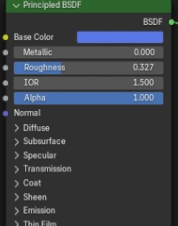
\includegraphics[width=0.4\linewidth]{col/15.png}
\end{figure}


\newpage
\subsection{Процесс моделирования 3-го объекта}

\subsubsection{Построение геомтерической модели}
\par \textbf{Шаг 1:} Добавляем в проект фотографию динозавра, которая послужит основой для моделирования. Для этого просто перетаскиваем фотографию из внешней папки в пространство проекта.
\begin{figure}[H]
    \label{4} 
    \centering
    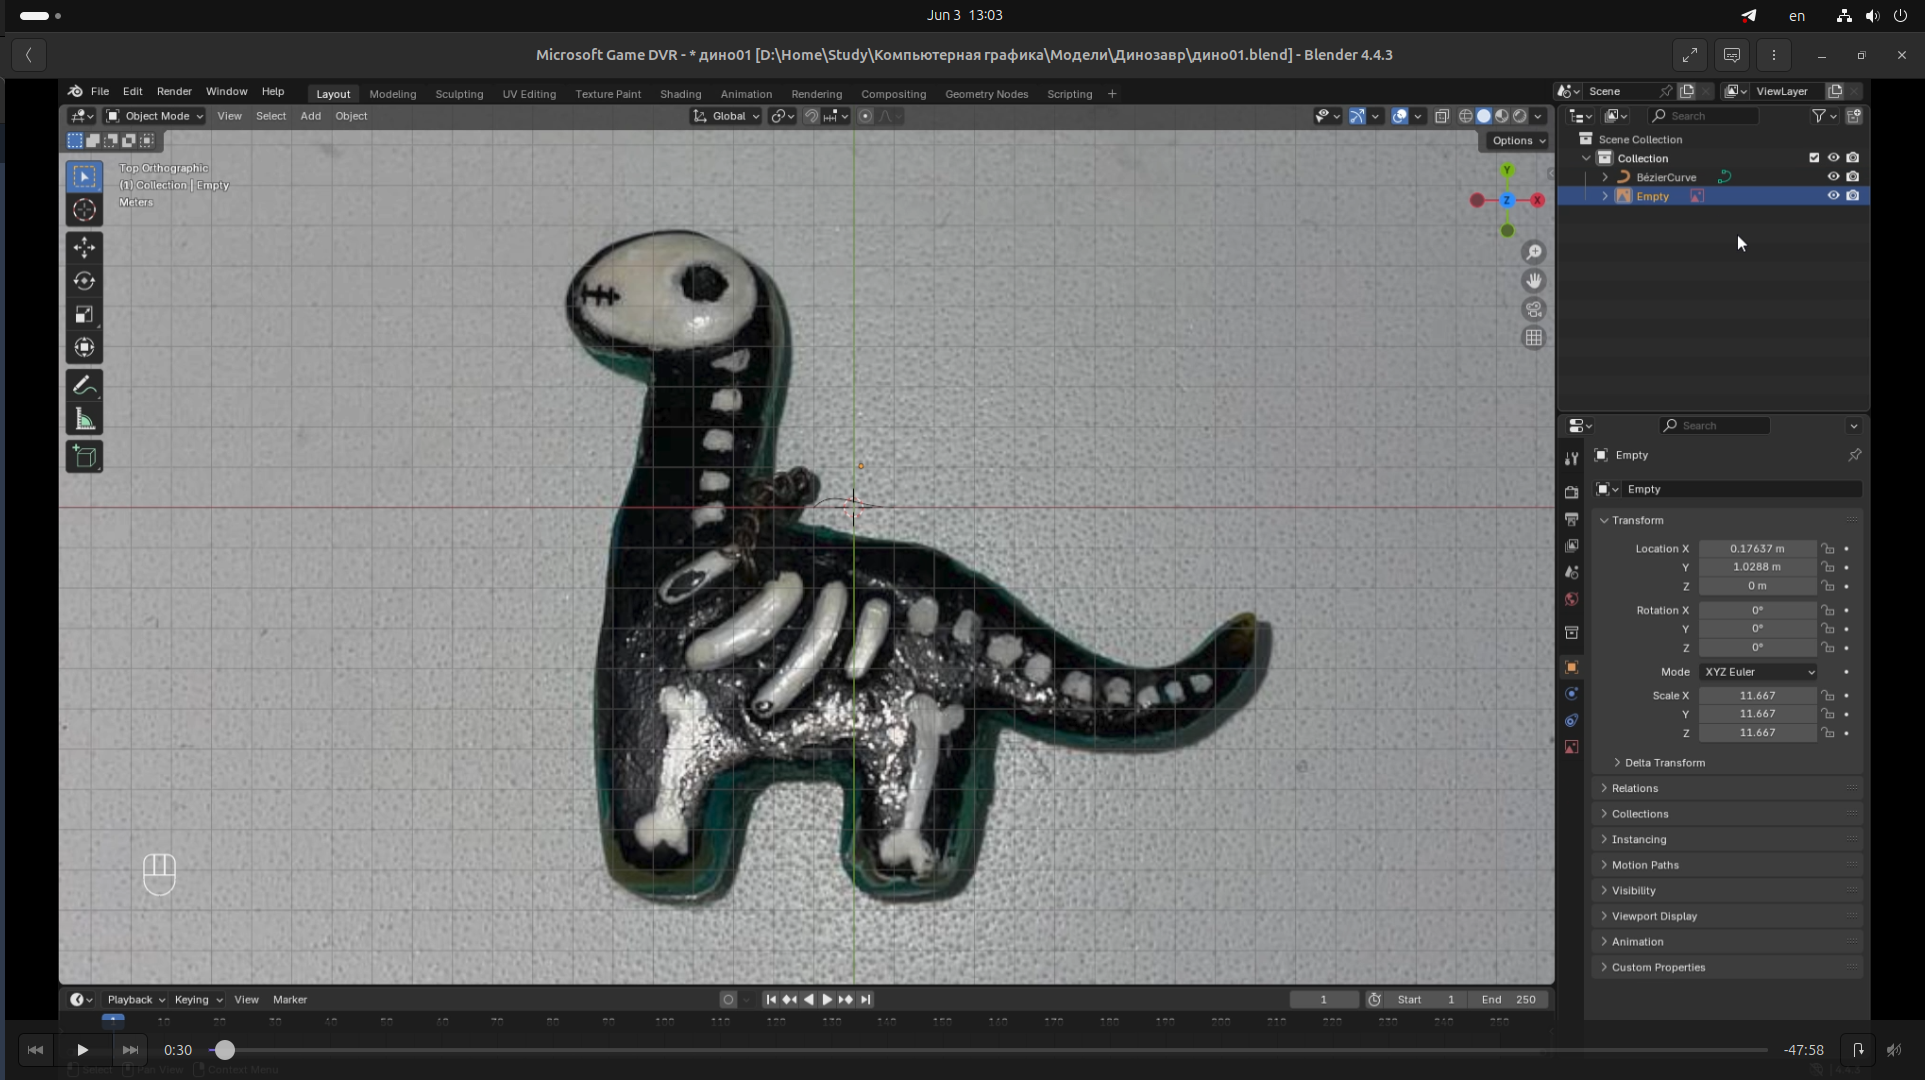
\includegraphics[width=0.8\linewidth]{dino/1.png}
    \caption{Шаг 1}
\end{figure}

\par \textbf{Шаг 2:} Для создания основы для формы динозавра создаём линию (\textit{Shift + A -> Mesh ->  Spline}) с параметром 'Vertex=18'. Затем необходимо расположить вершины (\textit{G+X+Y}) этой линии на местах изменения кривизны изначальной фигуры, что облегчит дальнейшую работу. 
\begin{figure}[H]
    \label{4} 
    \centering
    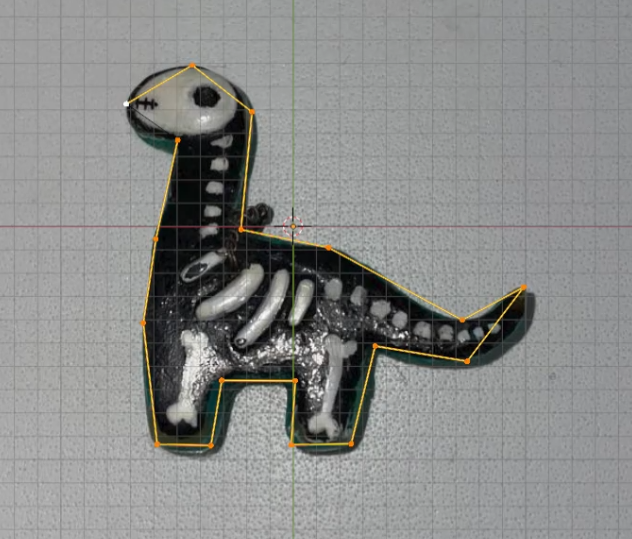
\includegraphics[width=0.6\linewidth]{dino/2.png}
    \caption{Шаг 2}
\end{figure}

\par \textbf{Шаг 3:} Выделяем все вершины (\textit{1+A}) и изменяем тип Spline на Bezier (\textit{ПКМ -> Set Spline Type -> Bezier}), что изменит линию с ломаной на кривую.
\begin{figure}[H]
    \label{4} 
    \centering
    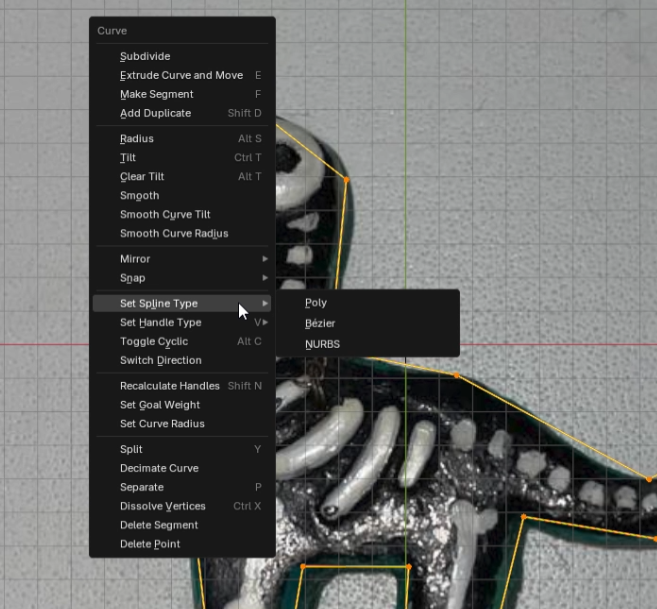
\includegraphics[width=0.6\linewidth]{dino/3.png}
    \caption{Шаг 3}
\end{figure}

\par \textbf{Шаг 4:} Вручную можно подкорректировать кривизну в отдельных вершинах (\textit{перемещение через ЛКМ}) для получения формы, максимально приближенной к форме фигурки.
\begin{figure}[H]
    \label{4} 
    \centering
    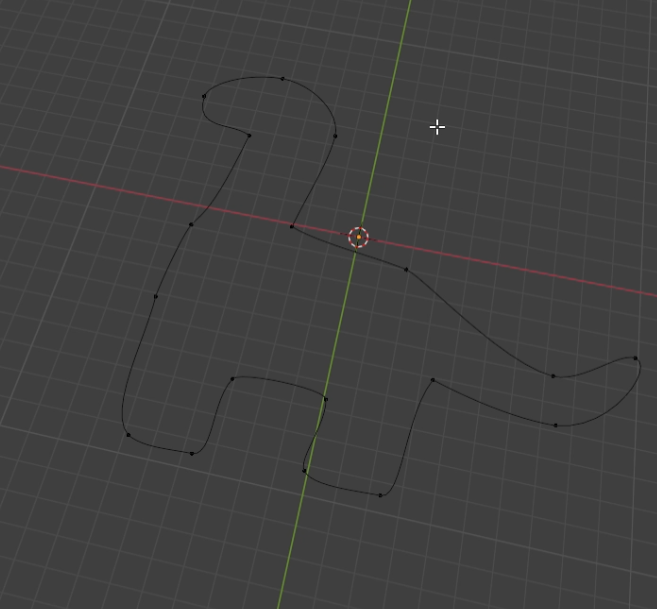
\includegraphics[width=0.6\linewidth]{dino/4.png}
    \caption{Шаг 4}
\end{figure}

\par \textbf{Шаг 5:} Для получения поверхности из полученной замкнутой кривой необходимо применить New Face from Edges (\textit{F}).
\begin{figure}[H]
    \label{4} 
    \centering
    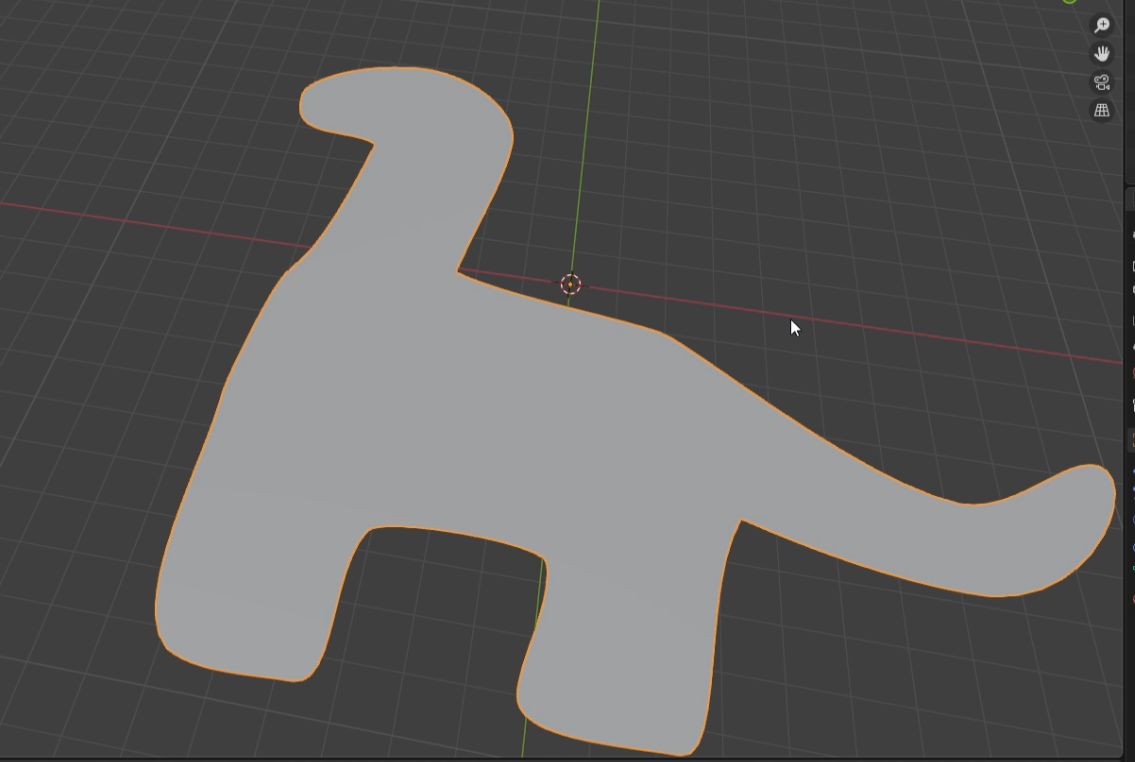
\includegraphics[width=0.6\linewidth]{dino/5.png}
    \caption{Шаг 5}
\end{figure}

\par \textbf{Шаг 6:} Для придания фигуре объёма применяем на него модификатор Extrude (\textit{E}).
\par Параметры модификатора:
\begin{itemize}
    \item Move X: 0
    \item Move Y: 0
    \item Move Z: 0.5m
\end{itemize}
\begin{figure}[H]
    \label{4} 
    \centering
    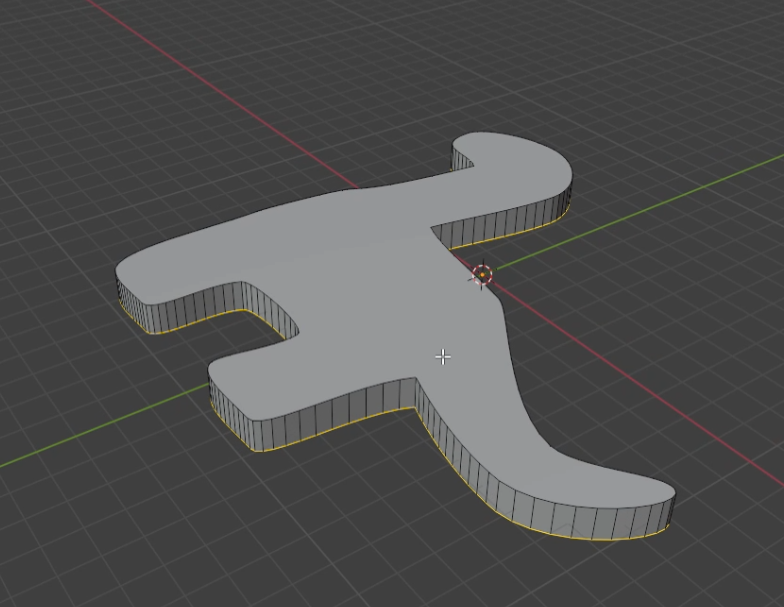
\includegraphics[width=0.6\linewidth]{dino/6.png}
    \caption{Шаг 6}
\end{figure}

\par \textbf{Шаг 7:} Выделяем верхние и нижние рёбра фигруки. Для придания более плавных форм и снятия фаски с этих вершин необходимо нажать комбинацию клавиш \textit{Ctrl+B} и задать следующие параметры:
\begin{itemize}
    \item Width: 0.112m
    \item Segments: 11
    \item Shape: 0.5
\end{itemize}
\begin{figure}[H]
    \label{4} 
    \centering
    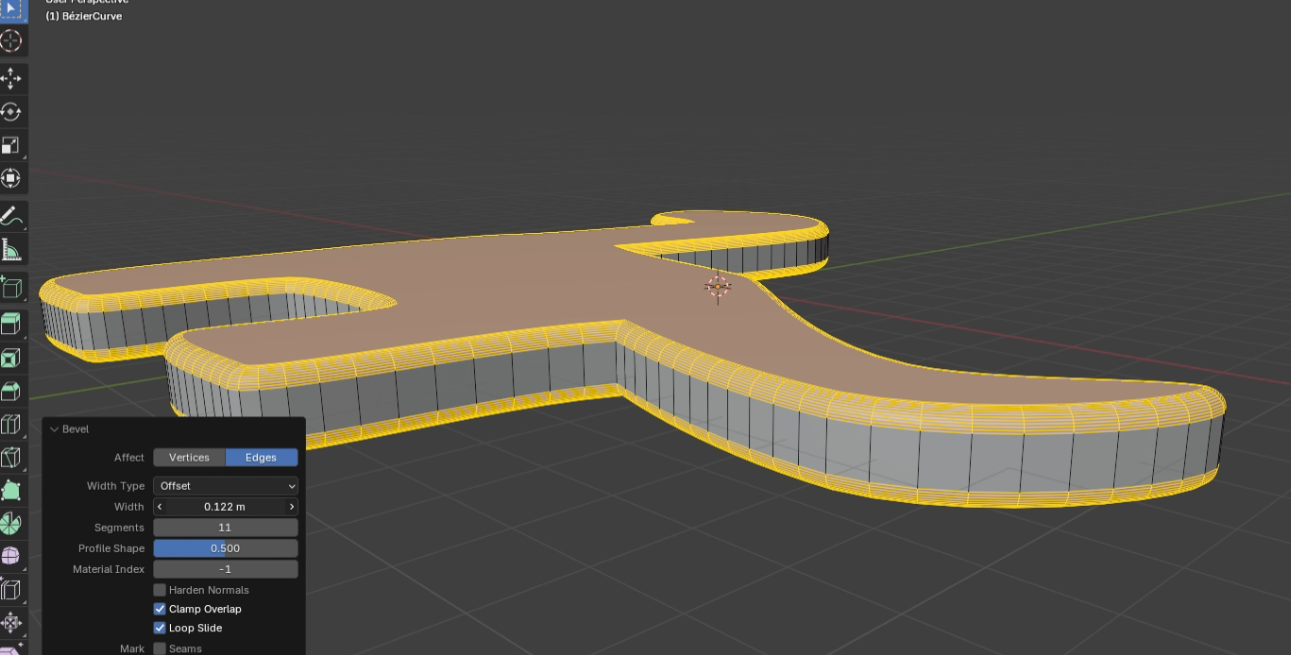
\includegraphics[width=0.8\linewidth]{dino/7.png}
    \caption{Шаг 7}
\end{figure}

\par \textbf{Шаг 8:} Открываем меню Добавить объект \textit{Shift + A -> Mesh ->  Cylinder} для создания отверстия для цепочки.
\begin{figure}[H]
    \label{4} 
    \centering
    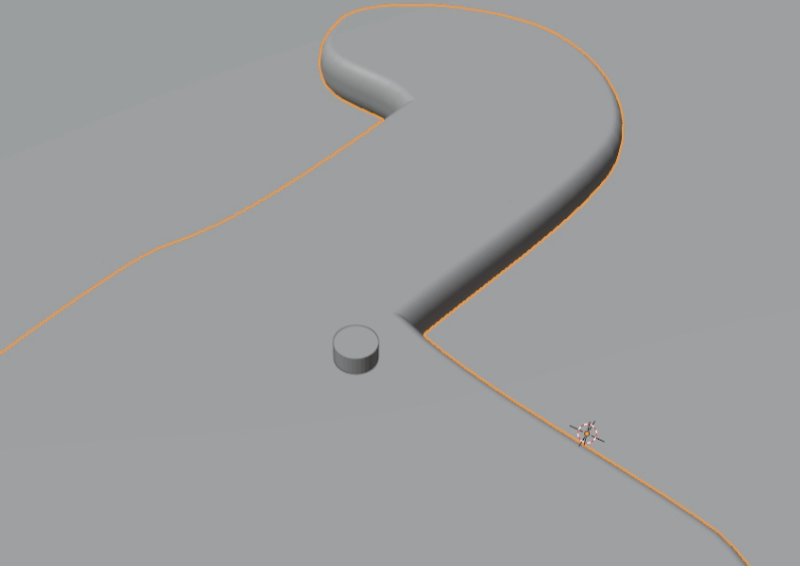
\includegraphics[width=0.8\linewidth]{dino/8.png}
    \caption{Шаг 8}
\end{figure}

\par \textbf{Шаг 9:} Для отверстия необходимо применить к фигурке и цилиндру модификатор Boolean (Difference).
\begin{figure}[H]
    \label{4} 
    \centering
    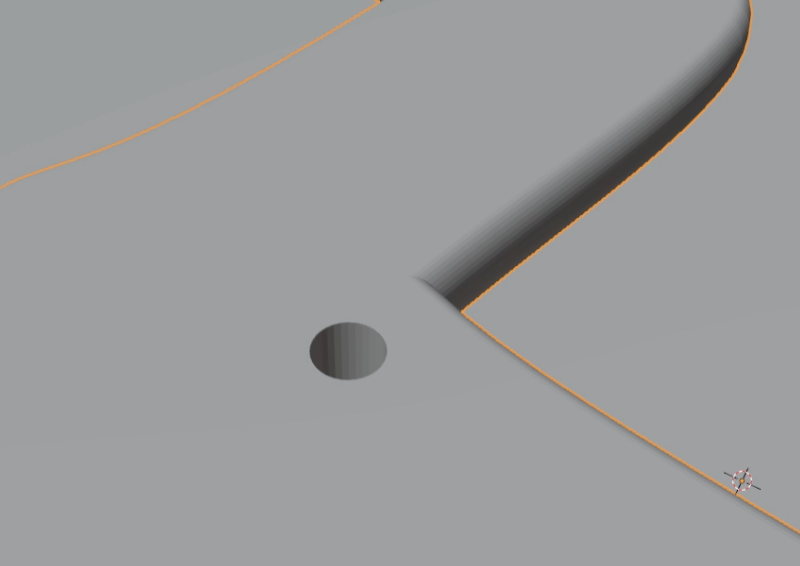
\includegraphics[width=0.8\linewidth]{dino/9.png}
    \caption{Шаг 9}
\end{figure}

\par \textbf{Шаг 10:} Для создания основы для цепочки, которая будет проходить через отверстие, создаём линию (\textit{Shift + A -> Mesh ->  Spline}) с параметром 'Vertex=10'. Затем необходимо расположить вершины (\textit{G+Z}) этой линии так, как бы вы хотели чтобы цепочка висела.
\begin{figure}[H]
    \label{4} 
    \centering
    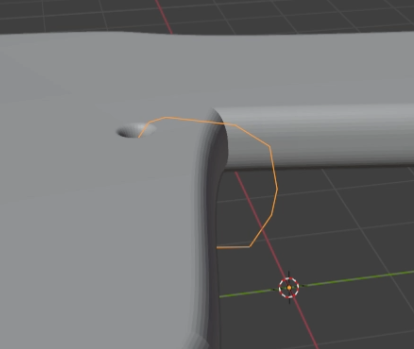
\includegraphics[width=0.8\linewidth]{dino/10.png}
    \caption{Шаг 10}
\end{figure}

\par \textbf{Шаг 11:} Для создания звена цепочки необходимо добавить объект Тор. Открываем меню Добавить объект \textit{Shift + A -> Mesh -> Torus} с параметрами
\begin{itemize}
    \item Major Segments: 125
    \item Minor Segments: 40
    \item Major Radius: 1m
    \item Minor Radius: 0.3m
\end{itemize}

\begin{figure}[H]
    \label{4} 
    \centering
    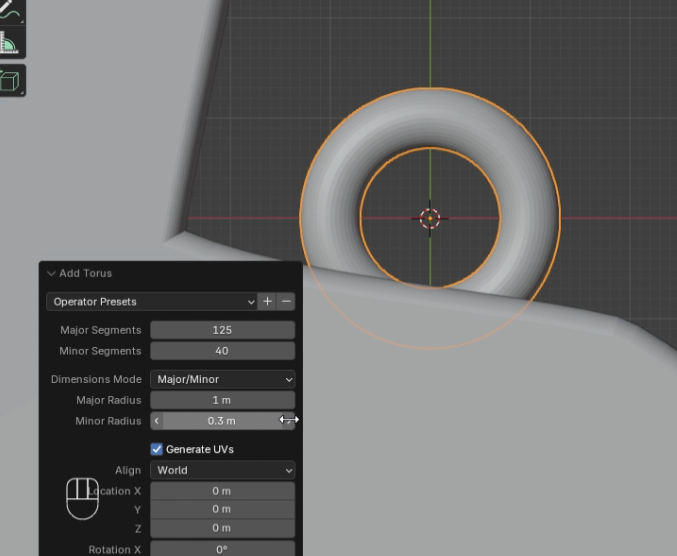
\includegraphics[width=0.8\linewidth]{dino/11.png}
    \caption{Шаг 11}
\end{figure}

\par \textbf{Шаг 12:} Для создания звена необходимо выделить половину полигонов и переместить их (\textit{G+X})

\begin{figure}[H]
    \label{4} 
    \centering
    \includegraphics[width=0.8\linewidth]{dino/12.png}
    \caption{Шаг 12}
\end{figure}


\par \textbf{Шаг 13:} Для создания цепочки необходимо к звену цепи применить модификаторы Array и Curve со следующими параметрами:

\begin{figure}[H]
    \label{4} 
    \centering
    \includegraphics[width=0.4\linewidth]{dino/13.2.png}
\end{figure}
Обязательно необходимо выбрать кривую, по которой будут располагаться звенья цепи!
\begin{figure}[H]
    \label{4} 
    \centering
    \includegraphics[width=0.8\linewidth]{dino/13.png}
    \caption{Шаг 13}
\end{figure}

\subsubsection{Добавление материала}
\par \textbf{Шаг 1:} Переходим в «Material properties» на панели инструментов → во вкладку «surface» → «Base color» → в поле «Set color» выберем из представленных наиболее похожий цвет на оригинальный цвет объекта, и следующие параметры:

\par \textbf{Черная часть динозавра}
\begin{enumerate}
    \item Metallic: 0.0
    \item Roughness: 0.409
    \item IOR: 1.5
\end{enumerate}

\begin{figure}[H]
    \label{4} 
    \centering
    \includegraphics[width=0.4\linewidth]{dino/14.png}
\end{figure}

\par \textbf{Зелёная часть динозавра}
\begin{enumerate}
    \item Metallic: 0.0
    \item Roughness: 0.232
    \item IOR: 1.5
\end{enumerate}

\begin{figure}[H]
    \label{4} 
    \centering
    \includegraphics[width=0.4\linewidth]{dino/15.png}
\end{figure}

\par \textbf{Цепь}
\begin{enumerate}
    \item Metallic: 0.350
    \item Roughness: 0.5
    \item IOR: 1.5
\end{enumerate}

\begin{figure}[H]
    \label{4} 
    \centering
    \includegraphics[width=0.4\linewidth]{dino/16.png}
\end{figure}


\par \textbf{Шаг 2:} Для добавления рисунка на модели необходимо во вкладке \textit{Shading} перейти в режим Paint на отображении UV развёртки текстуры Объекта. Где с помощью инструмента \textit{Кисть} необходимо нарисовать белым цветом рисунок.
\begin{figure}[H]
    \label{4} 
    \centering
    \includegraphics[width=0.8\linewidth]{dino/17.png}
\end{figure}


\newpage
\section{Результаты и сравнение с фотографией объекта}

\subsection{Результат и сравнение 1-ой модели с фотографией объекта}
На рисунке \ref{fig:pencilName} представлена фотография потертой надписи на карандаше.
На рисунке \ref{fig:pencilModel} представлена смоделированная часть карандаша (потертая надпись).

\begin{figure}[H]
    \centering
    \includegraphics[width=0.5\textwidth]{PencilName.png}
    \caption{Часть карандаша (потертая надпись)}
    \label{fig:pencilName}
\end{figure}

\begin{figure}[H]
    \centering
    \includegraphics[width=0.5\textwidth]{карандаш.png}
    \caption{Смоделированная часть карандаша (потертая надпись)}
    \label{fig:pencilModel}
\end{figure}

\subsection{Результат и сравнение 2-ой модели с фотографией объекта}
На рисунке \ref{fig:kolpakName} представлена фотография согнутого держателя колпака от авторучки.
На рисунке \ref{fig:kolpakModel} представлена смоделированная часть колпака от авторучки (согнутый держатель).

\begin{figure}[H]
    \centering
    \includegraphics[width=0.5\textwidth]{kolpak_org.png}
    \caption{Часть колпака от авторучки (согнутый держатель)}
    \label{fig:kolpakName}
\end{figure}

\begin{figure}[H]
    \centering
    \includegraphics[width=0.5\textwidth]{колпачок.png}
    \caption{Смоделированная часть колпака от авторучки (согнутый держатель)}
    \label{fig:kolpakModel}
\end{figure}

\subsection{Результат и сравнение 3-ой модели с фотографией объекта}
На рисунке \ref{fig:dinoName} представлена фотография игрушечного динозавра.
На рисунке \ref{fig:dinoModel} представлена смоделированная часть динозавра (игрушка сделанна собственноручно).
\begin{figure}[H]
    \centering
    \includegraphics[width=0.5\textwidth]{DinoFront.png}
    \caption{Часть динозавра (игрушка сделанна собственноручно)}
    \label{fig:dinoName}
\end{figure}

\begin{figure}[H]
    \centering
    \includegraphics[width=0.5\textwidth]{дино.png}
    \caption{Смоделированная часть динозавра (игрушка сделанна собственноручно)}
    \label{fig:dinoModel}
\end{figure}


\newpage
\section*{Заключение}
\addcontentsline{toc}{section}{Заключение}
\par В результате работы было сделано:
\begin{itemize}
    \item Получен навык работы с программным продуктом Blender.
    \item Были созданы трехмерные модели, повторяющие реальные объекты: Игрушечный динозавр, Колпак от авторучки, Карандаш.
    \item Была изучена технология посторения реалистической модели конкретных экземпляров
\end{itemize}


\newpage
\section*{Список литературы}
\addcontentsline{toc}{section}{Список литературы}
\begin{enumerate}
    \item  Болсуновская М.В. Компьютерная графика: Blender 3D: учеб. пособие / М.В.
Болсуновская, А.А Любченкова, В.В. Ракова. – СПб., 2021. – 118 с.
\end{enumerate}

\end{document}